\chapter{Testing}

Testing is intended to convey that an application does what it is intended to do, as well as to identify bugs before it is put into production. To test an application, you execute a program with artificial data before checking the results for errors, anomalies or information about the program's non-functional attributes \cite{sommerville}. The objective of carrying out tests can be categorised in two ways:

\paragraph{Validation Testing} To demonstrate to both the developer and customer that a software functions correctly and meets requirements. For bespoke, new software there should be a test performed for each requirement \cite{sommerville}.

\paragraph{Defect Testing} To identify bugs or defects in the application by finding inputs or input sequences where the behaviour of the software is unexpected, incorrect, undesirable or does not conform to requirements \cite{sommerville}. 

\begin{figure}[H]
    \centering
    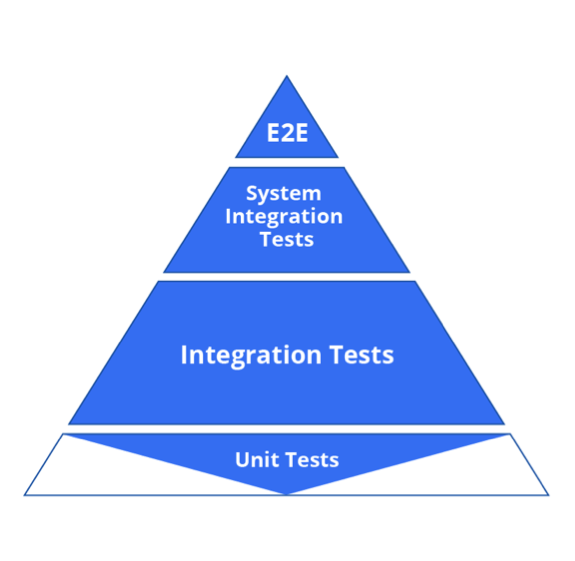
\includegraphics[width=0.5\textwidth]{9testing/images/testingDiagram.png}
    \caption{Agile pyramid of testing methods in the software development process \cite{pyramid2}.}
    \label{fig:testing}
\end{figure}

Figure \ref{fig:testing} shows the different testing methods in the software development process. They are ordered by their importance, since it can cost almost five times more to fix a coding defect once the system is released versus the cost in unit testing \cite{pyramid}. In the development of the codeHelper application, unit, end-to-end and integration testing were all performed to varying extents.

\section{Unit Testing}

A unit test exercises a `unit' of code in isolation and compares actual with expected results \cite{olan}. It is the process of testing the smallest components of a program, such as methods or object classes \cite{sommerville} - such as individual functions. Unit tests should call these functions with different input parameters. 

Unit testing was carried out in the development of codeHelper. Most unit testing was performed manually to test edge cases and correct functionality, however Jest \cite{jest} was also used to test the functionality of some units of the system.

\subsection{Jest}\label{sec:jest}

Jest is a JavaScript Testing Framework with a focus on simplicity \cite{jest}. It is a unit test framework that is built on top of Jasmine, supports the use of Typescript and is supported by React \cite{paul}.

In codeHelper, Jest was used to test the functionality of more complex utility functions. It also enabled tests to be written, saved and rerun whenever any changes had to be made - ensuring that no bugs were introduced. 
 
\section{Integration Testing}

Integration testing is a slight step up from unit testing. It involves the testing of multiple units that are integrated to form a larger unit. 

In the codeHelper application's development, methods or functions that were comprised of interactions between other functions were tested either manually or unit tested themselves - as discussed in section \ref{sec:jest}. 

\section{End-to-end Testing}

\gls{e2e} testing is a method which involves testing the workflow of an application from start to finish. The method does not require insight into the workings of the system, only the actual working of the application itself. The method is an attempt to replicate real life use cases so that the system requirements can be checked, known as requirement testing.

Requirements testing is an approach to test-case design where the requirements are used a basis to design tests. This is a form of validation testing \cite{sommerville}.

\subsection{Cypress}
In the development of the codeHelper application, Cypress \cite{cypress} was used to perform end-to-end requirements testing.

Cypress is a front end testing tool that enables the setting up, writing, running and debugging of tests \cite{cypress}. Cypress allowed testing using multiple browsers, viewport widths/screen sizes and speeds - however, its key features in the development of codeHelper were to allow E2E tests to be performed precisely, quickly and repeatedly throughout the development process. 

An example test is shown in figure \ref{fig:cyptest}. The test, titled `\textit{sets cookie and currentUser when logging in as lablead}', performs the following actions:

\begin{itemize}
    \item Visit the codeHelper site.
    \item Find the \textit{<div>} tag with id `username' and, within that div, find an input and type the lab lead username.
    \item Find the \textit{<div>} tag with id `password' and, within that div, find an input and type the lab lead password and enter to submit.
    \item \textbf{Check} that the site has redirected us correctly to the help desk page.
    \item \textbf{Check} that the site has set the correct cookie.
    \item Find the \textit{<a>} tag with id `currentUser' and \textbf{check} that it contains the lab lead username.
\end{itemize}

\begin{figure}[H]
    \begin{lstlisting}[frame=single]
it(`sets cookie and currentUser when logging in as lablead', function () {

    		cy.visit(`https://jm461.host.cs.st-andrews.ac.uk/labs/')

	    	cy.get(`div[id=username]').within(() => {
			    cy.get(`input').type(labLeadUsername)
		    })

	    	cy.get(`div[id=password]').within(() => {
		   	    cy.get(`input').type(`${labLeadPassword}{enter}`)
		   	})

		    cy.url().should(`include', `/demonstrator/desk')

		    cy.getCookie(`my_lil_cookie').should(`exist')

		    cy.get(`a[id=currentUser]').should(`contain', labLeadUsername)
	}) 
    \end{lstlisting}
        \caption{Cypress test code to check login functionality, correct setting of user and cookie.}
    \label{fig:cyptest}
\end{figure}

The Cypress test file is attached to the submission, titled `\textit{codeHelperTests.spec.js}'. The full results of some Cypress tests that were performed are shown in Figures \ref{fig:cyp1} and \ref{fig:cyp2}.

\begin{figure}[H]
    \centering
    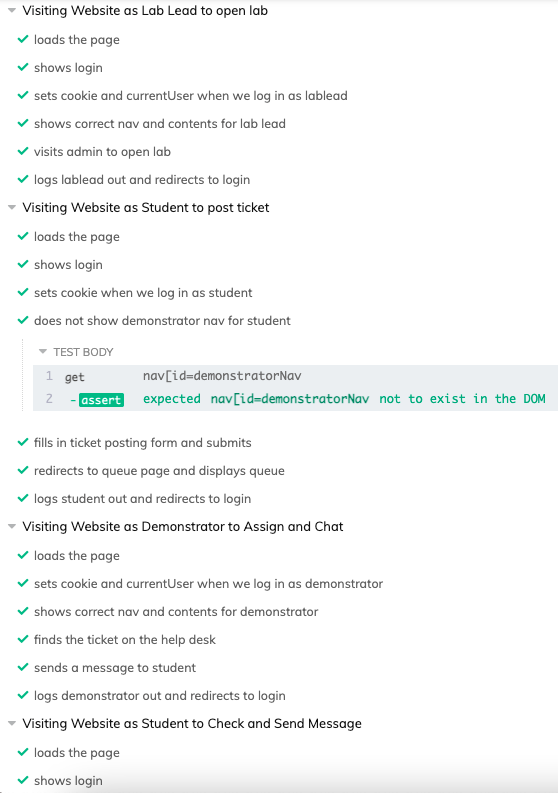
\includegraphics[width=0.75\textwidth]{9testing/images/cypress1.png}
    \caption{Cypress test results (Part 1).}
    \label{fig:cyp1}
\end{figure}

\begin{figure}[H]
    \centering
    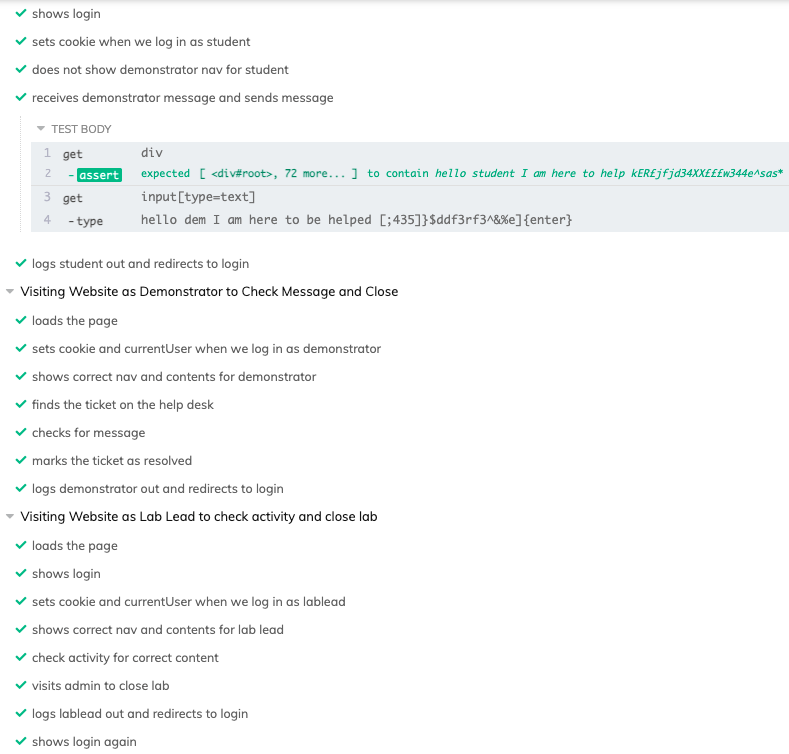
\includegraphics[width=\textwidth]{9testing/images/cypress2.png}
    \caption{Cypress test results (Part 2).}
    \label{fig:cyp2}
\end{figure}

\section{Manual Testing}

Manual testing sits on a level above the agile pyramid of testing methods shown in figure \ref{fig:testing}. It is less thorough and more expensive than other testing methods \cite{pyramid}, however is capable of detecting use cases arising from complex interaction that may be difficult to detect in earlier stages of testing.

Manual testing was also performed. It was carried out throughout development of the system. 
